\section{WIMP identification in Xenon}
\label{sec:wimps_with_xenon}

\par
The choice to build a detector using xenon is motivated by the A$^2$ enhancement in the scattering rate (\autoref{eq:wimp_si_differential_rate}).
Not only does the high atomic mass give good sensitivity to SI interactions, two naturally occurring xenon isotopes, ${}^{129}$Xe and ${}^{131}$Xe have a non-zero nuclear spin which makes them sensitive to SD interactions.
\par
The target medium (xenon) will have to be held in place by some other material.
This casing will contribute some amount of background due to radioactive impurities which will be observed as interactions in the target medium.
Xenon in liquid phase (LXe) is particularly good to counter this due to its high density (approximately 3g/cm${}^{3}$), and twinned with the large atomic mass has a high stopping power to both $\beta$ and $\gamma$ radioactive decays\footnote{for reference, aluminium has a density of 2.7 g/cm${}^{3}$}.
The inner volume of the the LXe medium will contain a very low background.

%Though the sensitivity to WIMP-proton spin-dependent interactions is less obvious as it requires neutron-proton mixing and is very dependent upon the nuclear model used.
%A further benefit of xenon is that it does not naturally contain any long-lived radioactive isotopes, or activation products.
%This means that the background rate is drive by 
%There are however several isotopes than can be produced by cosmogenically: and two metastable isotopes ${}^{129m}Xe$ and ${}^{131m}Xe$.


\subsection{Energy deposits in Xenon}
\par
An interaction of a particle within the target medium will result in either an interaction with the atomic nucleus, causing a nuclear recoil (NR), or within the electron cloud, resulting in a electron recoil (ER).
In both cases, the recoiling particle scatters with nearby atomic electrons and nuclei, transferring its kinetic energy: causing both excitation and ionisation of these atoms as a cascade of secondary recoils.
Regardless of which type of recoil occurs, an ionisation track is produced which culminates in scintillation light.
The reader is directed towards both \cite{xenon_physics_ref} and \cite{carldahl_thesis_ref} for thorough reviews of these processes, which are summarised below.
\par
An excited atom of xenon can bond to another xenon atom to form an excited molecule, or excimer, denoted as Xe$_2^{*\nu}$, which is both electronically and vibrationally excited.
This excimer will eventually vibrationally relax via collisions with other xenon atoms, and will decay to the ground state via the emission of a photon.
This process of excition luminescence, is shown below for an electronic recoil;
\begin{align*}
    e^- + Xe &\rightarrow Xe^* + e^+  &\text{impact excitation} \\ 
    Xe^* + Xe &\rightarrow Xe_2^{*,\nu} &\text{excimer formation} \\
    Xe_2^{*,\nu} + Xe &\rightarrow Xe_2^* + Xe &\text{relaxation} \\
    Xe_2^* &\rightarrow Xe + Xe + \gamma &\text{VUV emission} 
\end{align*}
An ionised atom can also produce scintillation light, though it's path to it is somewhat more complex.
The ionised atom can form diatomic molecules with nearby atoms.
Some of the electrons which were liberated during the cascade will recombine with the molecule, causing it to split leaving one of the atoms in a highly excited state (Xe$^{**}$).
The excited atom will then relax down, allowing for photon emission as before.
This process is referred to as recombination luminescence and is shown below for an electronic recoil;
\begin{align*}
    e^- + Xe &\rightarrow Xe^+ + 2e^+- &\text{ionisation} \\ 
    Xe^+ + Xe + Xe &\rightarrow Xe_2^{+} + Xe &\text{diatomic molecule formation} \\
    e^- + Xe_2^+ + Xe&\rightarrow Xe^{**} + Xe &\text{recombination} \\
    Xe^{**} + Xe &\rightarrow Xe^{*} + Xe + heat &\text{relaxation} \\
    Xe^{*} + Xe  &\rightarrow Xe_2^{*,\nu} &\text{excimer formation} \\
    Xe^{*} + Xe + Xe &\rightarrow Xe_2^{*} + Xe + heat &\text{relaxation} \\
    Xe_2^* &\rightarrow Xe + Xe + \gamma &\text{VUV emission} 
\end{align*}
\par
The difference in how these interactions appear between electronic recoils and nuclear recoils is shown in \autoref{fig:er_nr_tracks}.
From a nuclear recoil, the initial atom has a number of scatters, but these are typically below the ionisation level.
On the other hand, an electron recoil will result in a number of photons.
Additionally, as the electron is less stopped by the LXe, the track length is significantly greater.
If the interaction occurs in an electric field, not all of the electrons will recombine, allowing for potentially a second scintillation sighting.

\begin{figure}
    \centering
    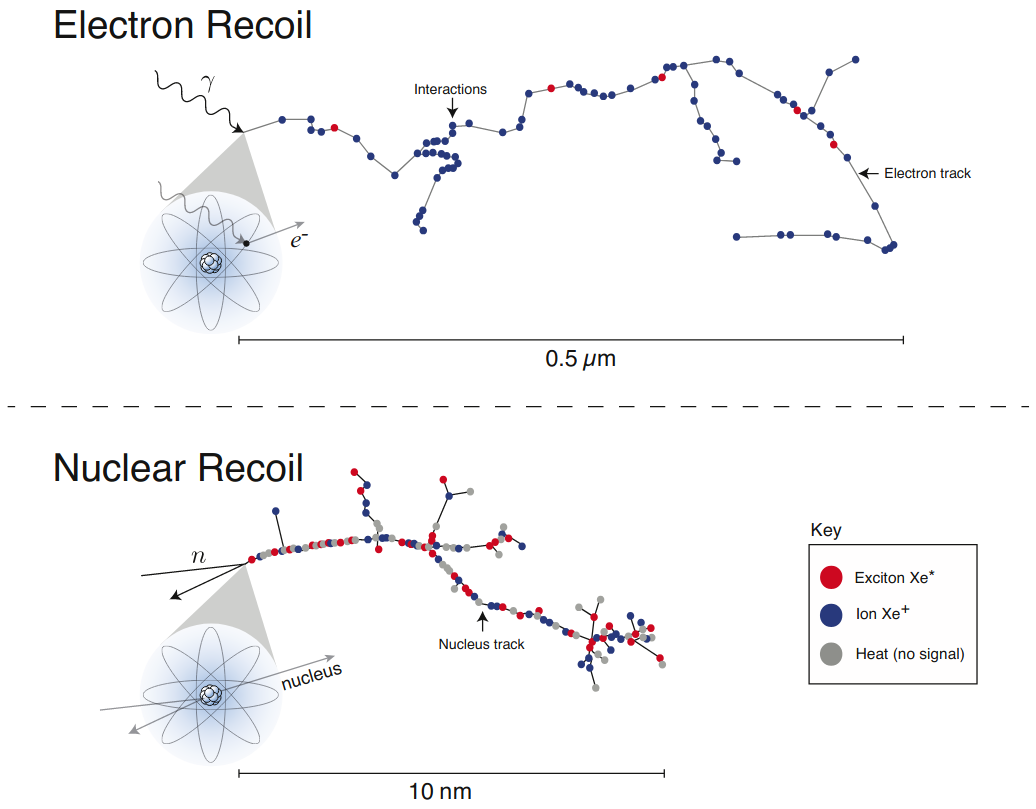
\includegraphics[width=\textwidth]{Figures/LZ/er_nr_tracks.png}
    \caption[Depiction of a 20keV recoil on liquid xenon]{Depiction of 20 keV recoil of electronic recoil (top) and nuclear recoil (bottom) in liquid xenon.
    Figure is from RIVAL simulations by C. Dahl \cite{carldahl_thesis_ref}, with adaptations by C. Fahan \cite{carlosfahan_thesis_ref}.}
    \label{fig:er_nr_tracks}
\end{figure}

\par
The energy deposited in LXe, is split between the atoms and liberated electrons, and so the energy of the recoil, E, can be written as:
\begin{equation}
    E = \frac{W}{L}(N_i + N_{ex})
\end{equation}
Here, W is the W-factor for LXe, generally taken to be 13.7 $\pm$ 0.2 eV \cite{light_and_charge_of_xenon_ref}, though there are more recent measurements indicating it could be as low as 11.5 eV \cite{electron_excitation_energy_of_xenon_ref}. 
N$_i$ and N$_{ex}$ are the number of ionised atoms and number of excited atoms respectively.
L corresponds to the ``Lindhard factor" or ``quenching" which accounts for the reduced light and charge that's lost to heat.
It is generally taken that L=1 for electron recoils as the heat loss does not vary with energy, allowing the impact this has to be taken into W.
\par
The ratio between the excitation atoms to ionisated atoms allows for ER and NR events to be distinguished, with the resultant number of photons observed differing between the two.
Experimentally, N$_{ex}$/N$_i$ has been measured as $\approx$ 1 for nuclear recoils, and 0.06 for electron recoils \cite{ionisation_to_excitation_ratio_xenon_ref}.

\subsection{Dual-phase Time Projection Chamber}
\par
One such detector design that can utilise the charge-to-light ratio between ER and NR signals are dual-phase time projection chambers (TPCs).
Modern variants of these detectors contain a single element in a majority liquid state with a region of gas above.
\par
An interaction event in a TPC is characterised by two signals.
Firstly a prompt scintillation signal in the liquid region - referred to as the S1.
This is caused by excimers and recombination previously discussed.
Secondly there is a delayed scintillation signal, or S2.
This is observed in the gas phase via electroluminescence.
Both of these signals produce VUV light ($\approx$175 nm) which can be detected by photomultipler tubes (PMTs) or silicon photomultipliers (SiPMs).
\par
In a typical TPC design, as shown in \autoref{fig:TPC_theory}, an electric field is applied.
This causes electrons that are freed as a result of the interaction to drift upwards towards the gas phase where there is a probability of being extracted into the gas phase and produce an S2 signal.
\par
With PMTs or SiPMs placed at both the top and bottom of the TPC, the size of the interaction signals can be measured.
The preferred unit of this is ``photons detected" (phd)\footnote{Historically the signal was measured in photoelectrons (phe) which can be traced back the to first TPC designs of the 1970s \cite{tpc_origins_ref}. However, as there is a non-negligible probability of two photoelectrons being emitted from a single VUV photon in a PMT \cite{pmts_in_xenon_ref}, phd has become more favourable as this can be taken into account.}.

\begin{figure}
    \centering
    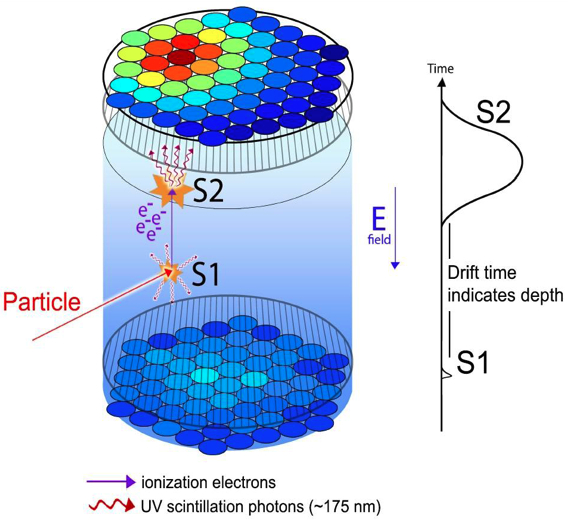
\includegraphics[width=0.6\textwidth]{Figures/LZ/tpc_theory.png}
    \caption{An illustration of the LUX dual-phase TPC \cite{lux_ref}.}
    \label{fig:TPC_theory}
\end{figure}

\par
The position of an interaction in the TPC can be reconstructed using only the S1 and S2 signals.
Firstly the $x-y$ position of an interaction can be reconstructed by the hit-pattern of photons on the gas phase PMTs. 
As the electrons will not deviate significantly from the interaction site while drifting, the hit-pattern is a good approximation of this location, with $\backsim$5 mm resolution demonstrated \cite{lux_position_reconstruction_ref}.
The $z$-position can be directly measured by the time difference between the two signals.
This is possible as the electrons reach a terminal drift velocity rapidly within the LXe, allowing for a resolution $\backsim$0.5 cm \cite{LZ_TechnicalDesignReview_ref}.
This high-resolution position reconstruction allows for the self-shielding of Xenon to be utilised by only selecting regions of LXe away from the TPC edge which will experiencing a significantly lower background rate.

\par
The size of the two pulses in terms of photons detected, which will now be referred to as S1 and S2, can be related to the underlying quanta which produced them via;
\begin{align}
    n_\gamma = N_{ex} + N_i r && n_e = N_i (1-r) \\
    S1 = n_\gamma G_1(x,y,z) && S2 = n_e G_2(x,y,z)
\end{align}
where both $G_1(x,y,z)$ and $G_2(x,y,z)$ account for the variable light collection efficiency.
It is useful to note that $G_1$ varies between 0 and 1 as the photons will not produce additional photons and so the maximum S1 can be is the number of photons produced.
On the other hand, $G_2$ can be greater than 1, as an extracted electron will produce more photons in the GXe.
In fact, $G_2$ is actually dependent upon the length of time an electron spends in the LXe, $t$, the efficiency the electron has to be extracted on the liquid surface, $\epsilon$, the scintillation yield in the gas phase, $Y_e$, and the light collection efficiency (LCE) in the gas $G_1^{gas}$.
The full expression of $G_2$ is give by:
\begin{equation}
    G_2 = e^{-t/\tau} \epsilon Y_e G_1^{gas}(x,y)
\end{equation}
In typical analysis, the S1 and S2 signals are manipulated to account for the change in LCE with position.
For this, two new quantities are introduced, as the corrected values: S1$_c$ and S2$_c$.
Both the S1 and S2 are adjusted to the centre of the TPC in \{$x,y$\}.
S1 is also adjusted to a $z$-position, typically taken to be the centre of the LXe.
\begin{align}
    S1_c = S1 \frac{G_1(0,0,z_c)}{G_1(x,y,z)} && S2_c = S2 \frac{G_1^{gas}(0,0)}{G_1^{gas}(x,y)} e^{t/\tau}
    \label{eq:s1c_and_s2c_full}
\end{align}
S1$_c$ and S2$_c$ are then just both linear relationships to the original quanta, related by a gain factor, $g$, which can be written as:
\begin{align}
    S1_c = g_1 n_\gamma && S2_c = g_2 n_e
\end{align}
With this linear relationship, the reconstructed recoil energy from the event of two pulses (and S1 and S2) becomes:
\begin{equation}
    E_R = \frac{W}{L}(\frac{S1_c}{g_1} + \frac{S2_c}{g_2})
\end{equation}
For NR events, L has an energy dependence.
\par
An example of the possible discrimination between ER and NR from a Xenon TPC is shown in \autoref{fig:er_nr_discrimination} for an arbitrary TPC detector.
The discrimination between ER and NR events is not perfect, with a non-negligible leakage between bands.
The viability of using TPCs for direct dark matter searches can be summarised by two requirements: understanding backgrounds and understanding ER and NR bands.

\begin{figure}[!htbp]%
\centering
\begin{tikzpicture}
\centering
    \begin{axis}[
            xlabel={S1${}_c$ [phd]},
            ylabel={log${}_{10}$ (S2${}_{c}$ [phd])},
            width=15cm, height=10cm,
            xmin=0, xmax=90,
            %ymin=0, %ymax=100,
            %minor y tick num=4,
            grid=major,]
            
            % ER Band
            \addplot[blue, opacity = 0.4, name path = er_high] table[x=x, y=high_er]
                {Data/tpc/bands.dat};
            \addplot[blue, opacity = 0.4, name path = er_low] table[x=x, y=low_er]
                {Data/tpc/bands.dat};
            \addplot[blue, opacity = 0.4] fill between[of=er_high and er_low];
            \addplot[blue, opacity = 0.8, name path = er_mid] table[x=x, y=mid_er]
                {Data/tpc/bands.dat};
            
            % NR Band
            \addplot[red, opacity = 0.4, name path = nr_high] table[x=x, y=high_nr]
                {Data/tpc/bands.dat};
            \addplot[red, opacity = 0.4, name path = nr_low] table[x=x, y=low_nr]
                {Data/tpc/bands.dat};
            \addplot[red, opacity = 0.4] fill between[of=nr_high and nr_low];
            \addplot[red, opacity = 0.8, name path = nr_mid] table[x=x, y=mid_nr]
                {Data/tpc/bands.dat};
            
            \addplot[blue, only marks,]
                   table [x=x,y=y]
              {Data/tpc/er_points.dat};
            \addplot[red, only marks,]
                   table [x=x,y=y]
              {Data/tpc/nr_points.dat};

    \end{axis}
\end{tikzpicture}
    \caption{Discrimination between electronic recoil (Blue) events and nuclear recoil (Red) events by the light-to-charge ratio.
             Simulations were performed by G. Rischbieter and additional details can be found in \cite{gregrischbieter_thesis_ref}}
    \label{fig:er_nr_discrimination}
\end{figure}

\par
Modelling of detector responses from S1 and S2 signals have undergone a huge amount of development in recent years, with the Noble Element Simulation Technique (NEST) library leading this.
Both Argon and Xenon detectors are modelled for energy deposits of sub-keV to several MeV \cite{nest_1_ref}.
Additional details of response modelling can be found in \cite{gregrischbieter_thesis_ref, flamenest_ref}.


\iffalse
\par


There are numerous different detector designs to choose from, and the reader is directed towards \cite{direct_detector_designs_ref} for an indepth comparison.


Fortunately, the majority of these will interact in the electron cloud surrounding the nucleus and result in an electronic recoil (ER).
This differs from the nuclear recoil (NR) which would be observed from a WIMP-nucleon interaction.
Therefore to detect a WIMP we are searching for an excess in NR events compared to out background.

\par
Therefore in order to achieve this, a target with minimal isotopes that will decay and cause an excess to be hidden need to be avoided.
Additionally, any detector design should allow for particle discrimination - or more explicit ER and NR discrimination. 
\fi